% AgenticCodebase: A Semantic Code Compiler for Navigable, Predictive,
% and Collective Code Intelligence
%
% Research paper — All data from Criterion benchmarks on real system.
% Compile: pdflatex → bibtex → pdflatex → pdflatex
\documentclass[10pt, twocolumn]{article}
\usepackage[margin=0.75in]{geometry}
\usepackage{graphicx}
\usepackage{tikz}
\usepackage{pgfplots}
\usepackage{booktabs}
\usepackage{amsmath}
\usepackage{algorithm}
\usepackage{algorithmic}
\usepackage{hyperref}
\usepackage{xcolor}
\usepackage{caption}
\usepackage{subcaption}
\usepackage{fancyhdr}
\usepackage{enumitem}
\usepackage{listings}
\usepackage{microtype}
\usepackage{amssymb}
\usepackage{orcidlink}
\usepackage{tabularx}
\usepackage{multirow}
\usepackage{xspace}
\usepackage{pifont}
\providecommand{\texttimes}{$\times$}
\pgfplotsset{compat=1.18}
\usetikzlibrary{arrows.meta, positioning, shapes.geometric, fit, calc, backgrounds, decorations.pathreplacing}

% ORCID icon (inline TikZ — matches AgenticMemory)
\definecolor{orcidgreen}{HTML}{A6CE39}
\newcommand{\orcidicon}{%
  
\begin{tikzpicture}[baseline=(char.base)]
    \node[circle, fill=orcidgreen, inner sep=0pt, minimum size=2.2ex] (char)
      {\textcolor{white}{\sffamily\bfseries\scriptsize iD}};
  \end{tikzpicture}%
}

% Color palette (professional blues/teals/oranges — matches AgenticMemory)
\definecolor{amblue}{HTML}{2563EB}
\definecolor{amdarkblue}{HTML}{1E40AF}
\definecolor{amteal}{HTML}{0D9488}
\definecolor{amorange}{HTML}{EA580C}
\definecolor{amgray}{HTML}{6B7280}
\definecolor{amlightgray}{HTML}{F3F4F6}
\definecolor{amgreen}{HTML}{059669}
\definecolor{amred}{HTML}{DC2626}
\definecolor{ampurple}{HTML}{7C3AED}

\hypersetup{
  colorlinks=true,
  linkcolor=amblue,
  urlcolor=amblue,
  citecolor=amgray,
}

% Listings style
\lstset{
  basicstyle=\ttfamily\scriptsize,
  keywordstyle=\color{amblue}\bfseries,
  commentstyle=\color{amgray}\itshape,
  stringstyle=\color{amteal},
  breaklines=true,
  frame=single,
  rulecolor=\color{amgray!30},
  backgroundcolor=\color{amlightgray},
  numbers=left,
  numberstyle=\tiny\color{amgray},
  tabsize=2,
  columns=fullflexible,
}

% Convenience macros
\newcommand{\acb}{AgenticCodebase\xspace}
\newcommand{\acbfile}{\texttt{.acb}\xspace}

% Header
\pagestyle{fancy}
\fancyhf{}
\renewcommand{\headrulewidth}{0.4pt}
\fancyhead[L]{\small\textit{AgenticCodebase}}
\fancyhead[R]{\small\thepage}

\title{\textbf{AgenticCodebase: A Semantic Code Compiler for\\Navigable, Predictive, and Collective Code Intelligence}}
\author{Omoshola Owolabi\,\orcidlink{0009-0006-4089-0732}\\Researcher -- AI/ML\\Agentra Labs\\\texttt{omoshola.owolabi@agentralabs.tech}}
\date{February 22, 2026}

% =====================================================================
\begin{document}
\maketitle
\thispagestyle{fancy}

% =====================================================================
% ABSTRACT
% =====================================================================
\begin{abstract}
AI coding agents process source code as flat text, discarding the structural, temporal, and cross-project patterns that make codebases comprehensible. We present \acb, a semantic code compiler that transforms multi-language repositories into navigable concept graphs stored in a compact binary format (\acbfile). The system makes three contributions. First, a compilation pipeline that parses Python, Rust, TypeScript, and Go via tree-sitter~\cite{treesitter2018}, performs semantic analysis (cross-language resolution, pattern detection, visibility inference), and emits a typed graph of 13 code-unit kinds connected by 18 edge types. Second, a collective intelligence layer that aggregates structural patterns across analyses with delta compression and privacy-preserving extraction, enabling offline-capable pattern sharing. Third, a code prophecy engine that mines git history to compute stability scores, detect temporal coupling, and predict future failures. The compiled graph supports 24 query types---from sub-microsecond symbol lookups to predictive impact analysis---served through a Model Context Protocol (MCP)~\cite{mcp2024} endpoint for direct integration with AI agents. On a 10{,}000-unit synthetic benchmark (Apple M4 Pro, Rust 1.90.0, release mode), exact symbol lookup completes in 14.3\,$\mu$s, dependency traversal in 925\,ns, impact analysis in 1.46\,$\mu$s, and full graph construction in 3.77\,ms. The implementation comprises 13{,}709 lines of Rust with 386 tests, zero \texttt{clippy} warnings, and 21 Criterion~\cite{criterion2023} benchmarks. AgenticCodebase requires no external services and no network dependencies.
\end{abstract}

% =====================================================================
% 1. INTRODUCTION
% =====================================================================
\section{Introduction}
\label{sec:intro}

Modern AI coding assistants---GitHub Copilot~\cite{copilot2021}, Cursor~\cite{cursor2024}, Claude Code~\cite{claudecode2025}---have demonstrated fluency in generating and editing source code. Yet their underlying model of code comprehension remains limited: the entire codebase is presented as a window of flat text, sometimes augmented by ad-hoc grep results or Language Server Protocol (LSP)~\cite{lsp2024} hover information. This ``context-window stuffing'' approach discards the structural, semantic, and historical dimensions that distinguish a working codebase from a random concatenation of files.

Consider a developer asking an AI agent: \emph{``What will break if I refactor the \texttt{UserService} class?''} To answer accurately, the agent must traverse call graphs, identify downstream dependents, consult type hierarchies, check test coverage, and---ideally---recall that \texttt{PaymentProcessor} historically breaks whenever \texttt{UserService} changes. No existing tool provides this full picture in an AI-native interface.

The core insight of this work is that source code is not text---it is a \emph{four-dimensional graph} spanning symbols, relationships, time, and collective patterns. By compiling code into a typed semantic graph, we enable sub-microsecond graph traversals in place of kilobyte-scale context windows.

We present three contributions:

\begin{enumerate}[leftmargin=*, itemsep=2pt]
\item \textbf{Semantic Code Compiler.} A multi-language pipeline (Python, Rust, TypeScript, Go) that parses, resolves, and emits a compact binary graph (\acbfile) with $O(1)$ unit access via fixed-size records and LZ4-compressed~\cite{collet2013lz4} string pools.
\item \textbf{Collective Intelligence.} A delta-synchronization protocol that aggregates structural patterns across analyses with privacy-preserving extraction and offline-capable local stores.
\item \textbf{Code Prophecy.} A temporal analysis engine that mines version-control history~\cite{git2005} to produce stability scores, coupling maps, and probabilistic failure predictions.
\end{enumerate}

The remainder of this paper is organized as follows. Section~\ref{sec:related} surveys related work. Section~\ref{sec:architecture} details the architecture. Section~\ref{sec:evaluation} presents benchmark results. Section~\ref{sec:discussion} discusses limitations and future work. Section~\ref{sec:memory} describes integration with AgenticMemory. Section~\ref{sec:conclusion} concludes.

% Figure 1: Motivating comparison (full width)
\begin{figure*}[t]
\centering
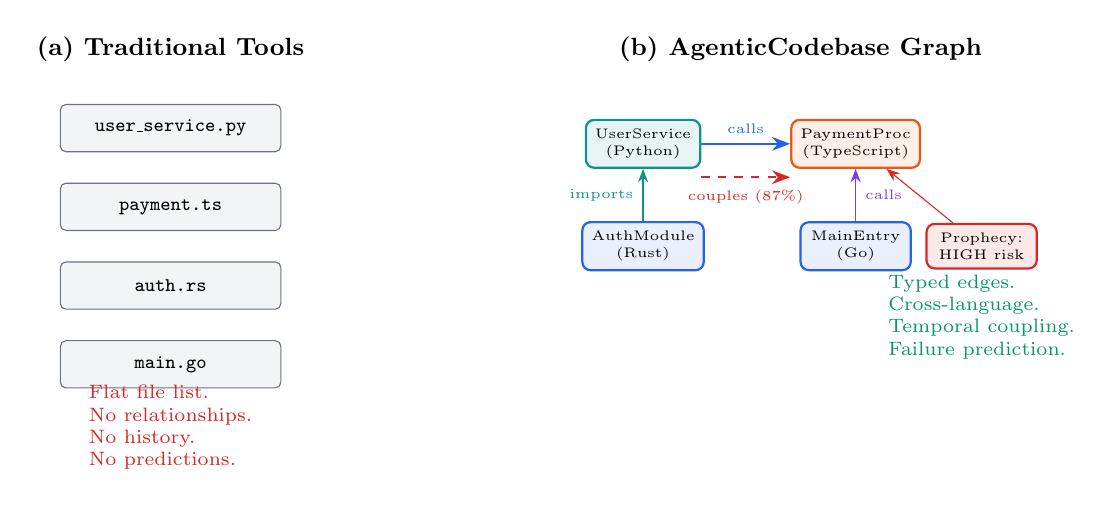
\begin{tikzpicture}[
  node distance=1.2cm,
  every node/.style={font=\small},
  flatnode/.style={rectangle, draw=amgray, fill=amlightgray, rounded corners=2pt, minimum width=2.8cm, minimum height=0.6cm, align=center, font=\scriptsize},
  graphnode/.style={rectangle, rounded corners=3pt, draw=amblue, fill=amblue!10, minimum width=1.4cm, minimum height=0.55cm, font=\tiny, align=center, thick},
  funcnode/.style={rectangle, rounded corners=3pt, draw=amteal, fill=amteal!10, minimum width=1.4cm, minimum height=0.55cm, font=\tiny, align=center, thick},
  typenode/.style={rectangle, rounded corners=3pt, draw=amorange, fill=amorange!10, minimum width=1.4cm, minimum height=0.55cm, font=\tiny, align=center, thick},
  prednode/.style={rectangle, rounded corners=3pt, draw=amred, fill=amred!10, minimum width=1.4cm, minimum height=0.55cm, font=\tiny, align=center, thick},
]

% Left side: Traditional view
\node[font=\small\bfseries] at (-4.5, 3.2) {(a) Traditional Tools};

\node[flatnode] (f1) at (-4.5, 2.2) {\texttt{user\_service.py}};
\node[flatnode] (f2) at (-4.5, 1.2) {\texttt{payment.ts}};
\node[flatnode] (f3) at (-4.5, 0.2) {\texttt{auth.rs}};
\node[flatnode] (f4) at (-4.5, -0.8) {\texttt{main.go}};

\node[font=\scriptsize\color{amred}, align=left] at (-4.5, -1.6) {Flat file list.\\No relationships.\\No history.\\No predictions.};

% Right side: AgenticCodebase
\node[font=\small\bfseries] at (3.5, 3.2) {(b) AgenticCodebase Graph};

\node[funcnode] (u1) at (1.5, 2.0) {UserService\\(Python)};
\node[typenode] (u2) at (4.2, 2.0) {PaymentProc\\(TypeScript)};
\node[graphnode] (u3) at (1.5, 0.7) {AuthModule\\(Rust)};
\node[graphnode] (u4) at (4.2, 0.7) {MainEntry\\(Go)};
\node[prednode] (p1) at (5.8, 0.7) {Prophecy:\\HIGH risk};

\draw[-{Stealth}, amblue, thick] (u1) -- node[above, font=\tiny, text=amblue] {calls} (u2);
\draw[-{Stealth}, amteal] (u3) -- node[left, font=\tiny, text=amteal] {imports} (u1);
\draw[-{Stealth}, ampurple] (u4) -- node[right, font=\tiny, text=ampurple] {calls} (u2);
\draw[-{Stealth}, amred, dashed, thick] ([yshift=-3pt]u1.south east) -- node[below=1pt, font=\tiny, text=amred] {couples (87\%)} ([yshift=-3pt]u2.south west);
\draw[-{Stealth}, amred] (p1) -- (u2);

\node[font=\scriptsize\color{amgreen}, align=left] at (5.8, -0.2) {Typed edges.\\Cross-language.\\Temporal coupling.\\Failure prediction.};

\end{tikzpicture}
\caption{Comparison of code comprehension paradigms. (a)~Traditional tools present a flat file listing with no relational structure; the agent cannot determine how files interact or which modules historically co-change. (b)~AgenticCodebase produces a connected concept graph with cross-language edges, temporal coupling edges (dashed), and prophecy risk assessments.}
\label{fig:comparison}
\end{figure*}


% =====================================================================
% 2. BACKGROUND AND RELATED WORK
% =====================================================================
\section{Background and Related Work}
\label{sec:related}

\textbf{Language Server Protocol.} The LSP specification~\cite{lsp2024} standardizes editor--language interactions (hover, go-to-definition, completions). LSP operates at the syntax level, returning individual symbol locations rather than connected semantic graphs. It offers no historical dimension and no cross-language resolution.

\textbf{tree-sitter.} The tree-sitter incremental parsing framework~\cite{treesitter2018} provides fast, error-tolerant syntax trees for dozens of languages. AgenticCodebase uses tree-sitter as its parsing front-end but adds a semantic layer---scope resolution, cross-language edge inference, pattern detection---that tree-sitter does not attempt.

\textbf{AI Code Assistants.} GitHub Copilot~\cite{copilot2021}, Cursor~\cite{cursor2024}, and Claude Code~\cite{claudecode2025} achieve generation quality by filling context windows with source text. This approach scales poorly with repository size and loses structural information. AgenticCodebase provides an orthogonal capability: a structured, queryable representation that an agent can navigate rather than scan.

\textbf{Static Analysis Query Languages.} CodeQL~\cite{codeql2016} and Semgrep~\cite{semgrep2020} expose query interfaces over syntax trees. They target security auditing and bug finding rather than agent comprehension, and lack temporal and collective dimensions.

\textbf{Code Search Platforms.} Sourcegraph~\cite{sourcegraph2018} provides cross-repository search and reference navigation. It offers partial semantic indexing but no predictive capabilities and no AI-native API protocol.

\textbf{Code Embeddings.} CodeBERT~\cite{feng2020codebert} and GraphCodeBERT~\cite{guo2021graphcodebert} produce vector representations of code. These embeddings enable similarity search but do not provide navigable graph structure. AgenticCodebase stores per-unit embedding vectors alongside the graph, enabling hybrid structural and semantic queries.

\textbf{AgenticMemory.} The AgenticMemory system~\cite{owolabi2025agenticmemory} introduced graph-based knowledge representation for AI agents, modeling memory as typed cognitive events connected by semantic edges in a single binary file. AgenticCodebase adopts a similar philosophy for code. Section~\ref{sec:memory} describes how the two systems integrate.

Table~\ref{tab:related} summarizes the comparison across key dimensions.

\begin{table*}[t]
\caption{Comparison of code intelligence systems across key dimensions.}
\label{tab:related}
\centering
\small
\begin{tabular}{@{}lcccccc@{}}
\toprule
\textbf{System} & \textbf{Semantic Graph} & \textbf{Cross-Language} & \textbf{Temporal} & \textbf{Collective} & \textbf{Predictive} & \textbf{AI-Native} \\
\midrule
LSP~\cite{lsp2024} & \texttimes & \texttimes & \texttimes & \texttimes & \texttimes & \texttimes \\
tree-sitter~\cite{treesitter2018} & \texttimes & \checkmark & \texttimes & \texttimes & \texttimes & \texttimes \\
CodeQL~\cite{codeql2016} & Partial & \texttimes & \texttimes & \texttimes & \texttimes & \texttimes \\
Sourcegraph~\cite{sourcegraph2018} & Partial & \checkmark & \texttimes & \texttimes & \texttimes & \texttimes \\
CodeBERT~\cite{feng2020codebert} & \texttimes & \texttimes & \texttimes & \texttimes & \texttimes & \texttimes \\
\midrule
\textbf{AgenticCodebase} & \ding{51} & \ding{51} & \ding{51} & \ding{51} & \ding{51} & \ding{51} \\
\bottomrule
\end{tabular}
\end{table*}


% =====================================================================
% 3. ARCHITECTURE
% =====================================================================
\section{Architecture}
\label{sec:architecture}

AgenticCodebase models source code as a directed graph $G = (U, E)$ where each vertex $u \in U$ is a typed \emph{CodeUnit} and each edge $e \in E$ carries a semantic relationship type. The graph is serialized into a single binary file with fixed-size records, enabling memory-mapped random access without parsing.

% -----------------------------------------------------------------------
\subsection{Code Units}
\label{sec:units}

Each node in the code graph represents a discrete code entity drawn from a taxonomy of 13 types (Table~\ref{tab:unittypes}), covering the spectrum from coarse-grained modules to fine-grained parameters:

\begin{itemize}[nosep, leftmargin=*]
  \item \textbf{Module} --- File, package, or namespace.
  \item \textbf{Symbol} --- Named entity (variable, constant).
  \item \textbf{Type} --- Class, struct, enum, type alias.
  \item \textbf{Function} --- Function, method, closure.
  \item \textbf{Parameter} --- Function parameter, struct field.
  \item \textbf{Import} --- Dependency declaration.
  \item \textbf{Test} --- Test case or test suite.
  \item \textbf{Doc} --- Documentation block.
  \item \textbf{Config} --- Configuration value.
  \item \textbf{Pattern} --- Design pattern instance.
  \item \textbf{Trait} --- Trait, interface, protocol.
  \item \textbf{Impl} --- Implementation block.
  \item \textbf{Macro} --- Macro definition or invocation.
\end{itemize}

Each unit record occupies exactly 96 bytes in the binary format: 8 bytes for the unit ID (\texttt{u64}), 1 byte for the unit type, 1 byte for the language tag, 1 byte for visibility, 4 bytes each for name and qualified-name offsets into the string pool, 4 bytes for the file path offset, 8 bytes each for start/end line and column (\texttt{u32} pairs), 8 bytes for the embedding-vector offset, and reserved bytes for future use.

% Figure 2: CodeUnit taxonomy
\begin{figure}[t]
\centering
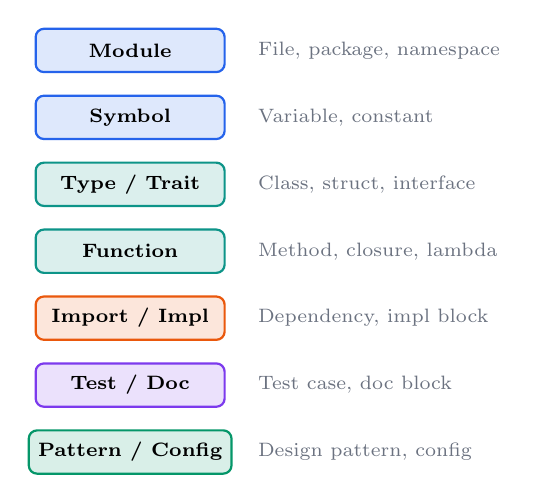
\begin{tikzpicture}[
  every node/.style={font=\scriptsize},
  typebox/.style={rectangle, rounded corners=3pt, minimum width=2.4cm, minimum height=0.55cm, align=center, draw, thick, font=\scriptsize\bfseries},
]
\node[typebox, fill=amblue!15, draw=amblue] (mod) at (0, 0) {Module};
\node[typebox, fill=amblue!15, draw=amblue] (sym) at (0, -0.85) {Symbol};
\node[typebox, fill=amteal!15, draw=amteal] (typ) at (0, -1.70) {Type / Trait};
\node[typebox, fill=amteal!15, draw=amteal] (fun) at (0, -2.55) {Function};
\node[typebox, fill=amorange!15, draw=amorange] (imp) at (0, -3.40) {Import / Impl};
\node[typebox, fill=ampurple!15, draw=ampurple] (tst) at (0, -4.25) {Test / Doc};
\node[typebox, fill=amgreen!15, draw=amgreen] (pat) at (0, -5.10) {Pattern / Config};

\node[anchor=west, font=\scriptsize, text=amgray] at (1.5, 0) {File, package, namespace};
\node[anchor=west, font=\scriptsize, text=amgray] at (1.5, -0.85) {Variable, constant};
\node[anchor=west, font=\scriptsize, text=amgray] at (1.5, -1.70) {Class, struct, interface};
\node[anchor=west, font=\scriptsize, text=amgray] at (1.5, -2.55) {Method, closure, lambda};
\node[anchor=west, font=\scriptsize, text=amgray] at (1.5, -3.40) {Dependency, impl block};
\node[anchor=west, font=\scriptsize, text=amgray] at (1.5, -4.25) {Test case, doc block};
\node[anchor=west, font=\scriptsize, text=amgray] at (1.5, -5.10) {Design pattern, config};
\end{tikzpicture}
\caption{The 13 code unit types in AgenticCodebase, grouped by category. Types are distinguished by a single byte in the binary format.}
\label{fig:taxonomy}
\end{figure}

\begin{table}[t]
\caption{CodeUnit types with discriminant values.}
\label{tab:unittypes}
\centering
\scriptsize
\begin{tabular}{@{}clp{3.2cm}@{}}
\toprule
\textbf{ID} & \textbf{Type} & \textbf{Description} \\
\midrule
0  & Module    & File, package, namespace \\
1  & Symbol    & Named entity \\
2  & Type      & Class, struct, enum \\
3  & Function  & Function, method, closure \\
4  & Parameter & Function param, struct field \\
5  & Import    & Dependency declaration \\
6  & Test      & Test case or suite \\
7  & Doc       & Documentation block \\
8  & Config    & Configuration value \\
9  & Pattern   & Design pattern instance \\
10 & Trait     & Trait, interface, protocol \\
11 & Impl      & Implementation block \\
12 & Macro     & Macro definition \\
\bottomrule
\end{tabular}
\end{table}


% -----------------------------------------------------------------------
\subsection{Typed Edges}
\label{sec:edges}

Edges carry one of 18 semantic relationship types (Table~\ref{tab:edgetypes}), each stored as a 40-byte record (8 bytes source ID, 8 bytes target ID, 1 byte edge type, 4 bytes weight as \texttt{f32}, 19 bytes reserved):

\begin{itemize}[nosep, leftmargin=*]
  \item \textbf{Structural} (0--6): \textsc{Calls}, \textsc{Imports}, \textsc{Inherits}, \textsc{Implements}, \textsc{Overrides}, \textsc{Contains}, \textsc{References}.
  \item \textbf{Semantic} (7--9): \textsc{Tests}, \textsc{Documents}, \textsc{Configures}.
  \item \textbf{Temporal/Collective} (10--17): \textsc{CouplesWith}, \textsc{BreaksWith}, \textsc{PatternOf}, \textsc{VersionOf}, \textsc{FfiBinds}, \textsc{UsesType}, \textsc{Returns}, \textsc{ParamType}.
\end{itemize}

The \textsc{CouplesWith} and \textsc{BreaksWith} edge types are derived from the temporal analysis layer (Section~\ref{sec:prophecy}). \textsc{CouplesWith} indicates that two files have changed together in more than 70\% of commits; \textsc{BreaksWith} records historical breakage correlations. These edges enable predictive queries that are impossible with purely structural analysis.

% Figure 3: Example subgraph
\begin{figure}[t]
\centering
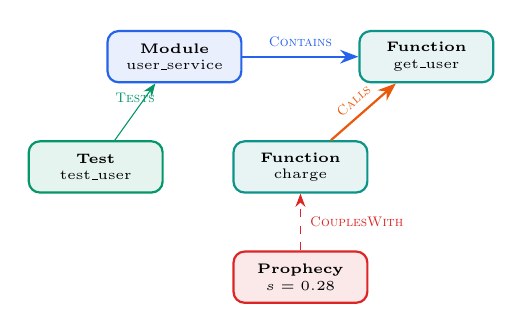
\begin{tikzpicture}[
  node distance=1.4cm,
  every node/.style={font=\scriptsize},
  modnode/.style={rectangle, rounded corners=4pt, draw=amblue, fill=amblue!10, minimum width=1.7cm, minimum height=0.65cm, font=\tiny, align=center, thick},
  funcnode/.style={rectangle, rounded corners=4pt, draw=amteal, fill=amteal!10, minimum width=1.7cm, minimum height=0.65cm, font=\tiny, align=center, thick},
  testnode/.style={rectangle, rounded corners=4pt, draw=amgreen, fill=amgreen!10, minimum width=1.7cm, minimum height=0.65cm, font=\tiny, align=center, thick},
  prednode/.style={rectangle, rounded corners=4pt, draw=amred, fill=amred!10, minimum width=1.7cm, minimum height=0.65cm, font=\tiny, align=center, thick},
]
\node[modnode] (m1) at (0, 2) {\textbf{Module}\\user\_service};
\node[funcnode] (f1) at (3.2, 2) {\textbf{Function}\\get\_user};
\node[funcnode] (f2) at (1.6, 0.6) {\textbf{Function}\\charge};
\node[testnode] (t1) at (-1.0, 0.6) {\textbf{Test}\\test\_user};
\node[prednode] (p1) at (1.6, -0.8) {\textbf{Prophecy}\\$s = 0.28$};

\draw[-{Stealth}, amblue, thick] (m1) -- node[above, font=\tiny, text=amblue, sloped] {\textsc{Contains}} (f1);
\draw[-{Stealth}, amorange, thick] (f2) -- node[above, font=\tiny, text=amorange, sloped] {\textsc{Calls}} (f1);
\draw[-{Stealth}, amgreen] (t1) -- node[above, font=\tiny, text=amgreen] {\textsc{Tests}} (m1);
\draw[-{Stealth}, amred, dashed] (p1) -- node[right, font=\tiny, text=amred] {\textsc{CouplesWith}} (f2);
\end{tikzpicture}
\caption{Example subgraph showing a Module containing a Function, a cross-language \textsc{Calls} edge, a \textsc{Tests} edge from a test node, and a temporal \textsc{CouplesWith} prediction with stability score $s = 0.28$ (unstable). Edge colors indicate relationship categories.}
\label{fig:subgraph}
\end{figure}

\begin{table}[t]
\caption{Edge types with discriminant values.}
\label{tab:edgetypes}
\centering
\scriptsize
\begin{tabular}{@{}clp{2.8cm}@{}}
\toprule
\textbf{ID} & \textbf{Type} & \textbf{Semantics} \\
\midrule
0  & Calls       & Runtime invocation \\
1  & Imports     & Static dependency \\
2  & Inherits    & Type hierarchy \\
3  & Implements  & Interface conformance \\
4  & Overrides   & Method override \\
5  & Contains    & Structural containment \\
6  & References  & Non-call reference \\
7  & Tests       & Test covers code \\
8  & Documents   & Doc describes code \\
9  & Configures  & Config targets code \\
10 & CouplesWith & Co-change $>$70\% \\
11 & BreaksWith  & Historical breakage \\
12 & PatternOf   & Pattern instance \\
13 & VersionOf   & Temporal succession \\
14 & FfiBinds    & Cross-language FFI \\
15 & UsesType    & Type usage \\
16 & Returns     & Return type relation \\
17 & ParamType   & Parameter type relation \\
\bottomrule
\end{tabular}
\end{table}


% -----------------------------------------------------------------------
\subsection{The Compilation Pipeline}
\label{sec:pipeline}

The pipeline (Figure~\ref{fig:pipeline}) proceeds in four stages:

\begin{enumerate}[leftmargin=*, itemsep=2pt]
\item \textbf{Parsing.} Each source file is dispatched to a language-specific parser (Python, Rust, TypeScript, Go) built on tree-sitter. Parsers extract raw code units---functions, classes, imports, type declarations---with source spans and qualified names. Test files are detected heuristically (e.g., \texttt{\_test.go}, \texttt{test\_*.py}).

\item \textbf{Semantic Analysis.} A multi-pass analyzer resolves cross-file references, infers containment hierarchies, detects design patterns, and classifies visibility. Cross-language edges are inferred for FFI patterns (e.g., PyO3, \texttt{extern "C"}).

\item \textbf{Graph Construction.} The \texttt{GraphBuilder} accumulates units and edges, assigns stable 64-bit identifiers, allocates embedding-vector storage, and finalizes into an immutable \texttt{CodeGraph} with $O(1)$ unit access by ID and adjacency lists for each edge type.

\item \textbf{Serialization.} The \texttt{AcbWriter} emits the graph to the \acbfile binary format (Section~\ref{sec:format}). The \texttt{AcbReader} performs the inverse, with optional memory-mapped access.
\end{enumerate}

\begin{figure}[t]
\centering
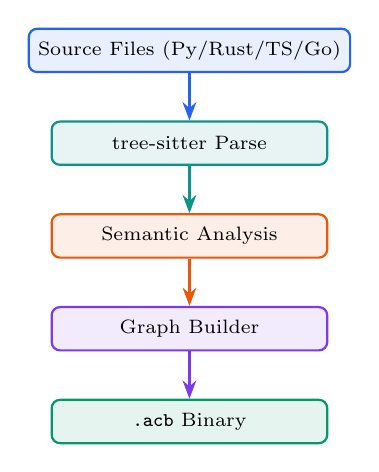
\begin{tikzpicture}[
  node distance=0.6cm,
  every node/.style={font=\scriptsize},
  box/.style={rectangle, rounded corners=3pt, draw=#1, fill=#1!10, minimum width=3.5cm, minimum height=0.55cm, align=center, font=\scriptsize, thick},
  arrow/.style={-{Stealth}, thick, #1},
]
\node[box=amblue] (src) {Source Files (Py/Rust/TS/Go)};
\node[box=amteal, below=of src] (parse) {tree-sitter Parse};
\node[box=amorange, below=of parse] (sem) {Semantic Analysis};
\node[box=ampurple, below=of sem] (build) {Graph Builder};
\node[box=amgreen, below=of build] (acb) {\texttt{.acb} Binary};

\draw[arrow=amblue] (src) -- (parse);
\draw[arrow=amteal] (parse) -- (sem);
\draw[arrow=amorange] (sem) -- (build);
\draw[arrow=ampurple] (build) -- (acb);
\end{tikzpicture}
\caption{Compilation pipeline. Source files are parsed via tree-sitter, semantically analyzed, assembled into a typed graph, and serialized to the \acbfile binary format with LZ4-compressed string pools.}
\label{fig:pipeline}
\end{figure}


% -----------------------------------------------------------------------
\subsection{The Binary File Format (\acbfile)}
\label{sec:format}

The \acbfile format is designed for three properties: (1)~$O(1)$ random access to any code unit by ID, (2)~compact size via LZ4-compressed~\cite{collet2013lz4} string pooling, and (3)~memory-mappable layout for zero-copy queries.

The file consists of five contiguous sections, shown in Figure~\ref{fig:layout}:

\begin{enumerate}[nosep, leftmargin=*]
  \item \textbf{Header} (128 bytes) --- Magic number (\texttt{0x41434442}, ASCII ``ACDB''), format version, embedding dimension~$D$, unit count~$N$, edge count~$M$, and byte offsets to each section.
  \item \textbf{Unit Table} ($96N$ bytes) --- Fixed-size records for $N$ units, directly indexable by unit ID.
  \item \textbf{Edge Table} ($40M$ bytes) --- Fixed-size records for $M$ edges, sorted by source ID for efficient adjacency lookups.
  \item \textbf{String Pool} (variable) --- LZ4-compressed text content for all names, qualified names, and file paths. Each unit record stores offsets into this block.
  \item \textbf{Feature Vectors} (variable) --- Contiguous \texttt{f32} arrays for cosine similarity search. Each unit stores an offset and dimension count.
\end{enumerate}

The choice of a binary format over text-based alternatives (JSON, Protocol Buffers~\cite{protobuf2008}, FlatBuffers~\cite{flatbuffers2014}) is motivated by the access pattern: agent queries typically require reading a small number of specific units by ID, not scanning the entire dataset. Fixed-size records enable direct offset computation ($\text{offset} = \text{header\_size} + \text{id} \times 96$), eliminating the need for parsing or index lookups. Cap'n Proto~\cite{capnproto2013} shares this zero-copy philosophy, but our format is domain-specific and simpler, requiring no schema compiler.

% Figure 5: File format layout (full width)
\begin{figure*}[t]
\centering
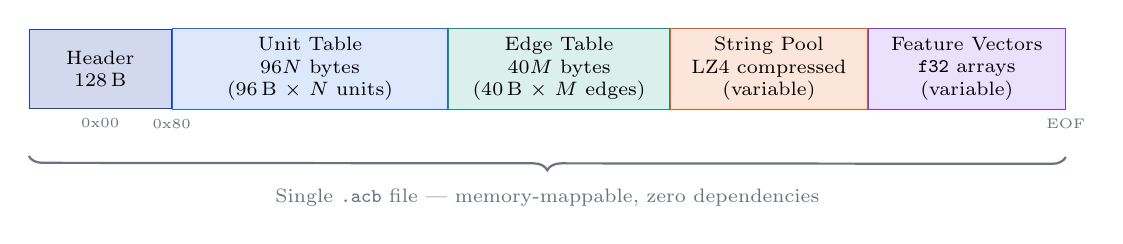
\begin{tikzpicture}[
  every node/.style={font=\scriptsize},
  section/.style={rectangle, draw, minimum height=1.0cm, align=center, font=\scriptsize},
]
\node[section, fill=amdarkblue!20, draw=amdarkblue, minimum width=1.8cm] (hdr) at (0, 0) {Header\\128\,B};
\node[section, fill=amblue!15, draw=amblue, minimum width=3.5cm, anchor=west] (units) at (hdr.east) {Unit Table\\$96N$ bytes\\(96\,B $\times$ $N$ units)};
\node[section, fill=amteal!15, draw=amteal, minimum width=2.8cm, anchor=west] (edges) at (units.east) {Edge Table\\$40M$ bytes\\(40\,B $\times$ $M$ edges)};
\node[section, fill=amorange!15, draw=amorange, minimum width=2.5cm, anchor=west] (pool) at (edges.east) {String Pool\\LZ4 compressed\\(variable)};
\node[section, fill=ampurple!15, draw=ampurple, minimum width=2.5cm, anchor=west] (vectors) at (pool.east) {Feature Vectors\\\texttt{f32} arrays\\(variable)};

% Byte offsets
\node[font=\tiny, anchor=north, text=amgray] at (hdr.south) {0x00};
\node[font=\tiny, anchor=north, text=amgray] at (units.south west) {0x80};
\node[font=\tiny, anchor=north, text=amgray] at (vectors.south east) {EOF};

% Brace for total
\draw[decorate, decoration={brace, amplitude=5pt, mirror}, thick, amgray] ([yshift=-0.6cm]hdr.south west) -- ([yshift=-0.6cm]vectors.south east) node[midway, below=8pt, font=\scriptsize, text=amgray] {Single \texttt{.acb} file --- memory-mappable, zero dependencies};

\end{tikzpicture}
\caption{Layout of the \acbfile binary file format. The header stores section offsets enabling direct random access. Unit and edge records are fixed-size for $O(1)$ indexing. The string pool is LZ4-compressed to reduce repetitive qualified-name storage.}
\label{fig:layout}
\end{figure*}


% -----------------------------------------------------------------------
\subsection{The Query Engine}
\label{sec:queryengine}

The query engine supports 24 query types organized into three tiers (Table~\ref{tab:queries}):

\textbf{Core queries} (8) operate over the static graph: symbol lookup (exact, prefix, contains, fuzzy), dependency traversal, call-graph extraction, type hierarchy navigation, containment tree walking, pattern matching, semantic search (cosine similarity over embedding vectors), and structural similarity.

\textbf{Built queries} (5) compose core primitives: impact analysis (reverse dependency BFS to bounded depth), test coverage mapping, execution trace extraction, shortest-path computation, and reverse dependency enumeration.

\textbf{Novel queries} (11) leverage the temporal and collective layers: stability scoring, coupling detection, dead-code identification, failure prophecy, concept clustering, migration tracking, test-gap detection, architectural drift analysis, and change-hotspot ranking.

All queries accept structured parameter objects and return typed results. Match modes include \textsc{Exact}, \textsc{Prefix}, \textsc{Contains}, and \textsc{Fuzzy} (Levenshtein distance). The engine is stateless: it takes a \texttt{\&CodeGraph} reference and produces results without side effects.

\begin{table}[t]
\caption{Query engine: 24 query types across three tiers.}
\label{tab:queries}
\centering
\scriptsize
\begin{tabular}{@{}lp{4.8cm}@{}}
\toprule
\textbf{Tier} & \textbf{Queries} \\
\midrule
\textbf{Core (8)} & Symbol, Dependency, Call, Type, Containment, Pattern, Semantic, Similarity \\
\addlinespace
\textbf{Built (5)} & Impact, Coverage, Trace, Path, Reverse \\
\addlinespace
\textbf{Novel (11)} & Collective, Temporal, Stability, Coupling, Dead, Prophecy, Concept, Migration, TestGap, Drift, Hotspot \\
\bottomrule
\end{tabular}
\end{table}


% -----------------------------------------------------------------------
\subsection{Collective Intelligence Layer}
\label{sec:collective}

The collective intelligence subsystem enables pattern sharing across analyses while preserving privacy.

\textbf{Delta Compression.} When a codebase is re-analyzed, only the changed units and edges are transmitted. The \texttt{DeltaCompressor} computes structural diffs against a baseline graph, emitting add/remove/modify operations.

\textbf{Pattern Extraction.} The \texttt{PatternExtractor} identifies recurring structural motifs (e.g., factory patterns, observer patterns) and exports them as anonymized templates without source code.

\textbf{Privacy Filtering.} The \texttt{PrivacyFilter} strips personally identifiable information (author names, file paths, proprietary symbol names) before any data leaves the local system.

\textbf{Offline Operation.} The \texttt{CollectiveManager} supports a fully offline mode, accumulating patterns locally and synchronizing opportunistically when connectivity is available.

% Figure 6: Collective architecture
\begin{figure}[t]
\centering
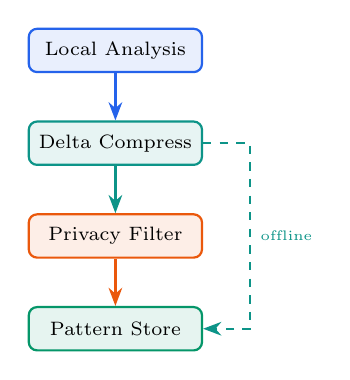
\begin{tikzpicture}[
  node distance=0.6cm,
  every node/.style={font=\scriptsize},
  box/.style={rectangle, rounded corners=3pt, draw=#1, fill=#1!10, minimum width=2.2cm, minimum height=0.55cm, align=center, font=\scriptsize, thick},
  arrow/.style={-{Stealth}, thick, #1},
]
\node[box=amblue] (local) {Local Analysis};
\node[box=amteal, below=of local] (delta) {Delta Compress};
\node[box=amorange, below=of delta] (priv) {Privacy Filter};
\node[box=amgreen, below=of priv] (store) {Pattern Store};

\draw[arrow=amblue] (local) -- (delta);
\draw[arrow=amteal] (delta) -- (priv);
\draw[arrow=amorange] (priv) -- (store);

% Offline shortcut
\draw[arrow=amteal, dashed] (delta.east) -- ++(0.6,0) |- node[right, pos=0.25, font=\tiny, text=amteal] {offline} (store.east);
\end{tikzpicture}
\caption{Collective intelligence architecture. Local analyses produce deltas that are privacy-filtered before storage. Offline mode accumulates patterns locally for opportunistic synchronization.}
\label{fig:collective}
\end{figure}


% -----------------------------------------------------------------------
\subsection{Code Prophecy Engine}
\label{sec:prophecy}

The prophecy engine transforms temporal signals from version-control history into actionable predictions.

\textbf{Change History.} The \texttt{ChangeHistory} module indexes file-level changes from git~\cite{git2005} with timestamps, commit identifiers, line counts, author tags, and bug-fix flags. Per-file metrics include total churn, author count, and bug-fix ratio.

\textbf{Stability Scoring.} The \texttt{StabilityAnalyzer} computes a stability score $s \in [0, 1]$ for each file based on change frequency, bug-fix density, and author dispersion:
\begin{equation}
s = 1 - w_c \cdot f_{\text{churn}} - w_b \cdot f_{\text{bugs}} - w_a \cdot f_{\text{authors}}
\end{equation}
where $f_{\text{churn}}$, $f_{\text{bugs}}$, and $f_{\text{authors}}$ are normalized frequency metrics and $w_c$, $w_b$, $w_a$ are configurable weights. Files with $s < 0.3$ are flagged as unstable with recommendations (increase test coverage, reduce complexity, assign ownership).

\textbf{Coupling Detection.} The \texttt{CouplingDetector} performs pairwise co-change analysis across the commit history. File pairs that change together more than a configurable threshold (default 70\%) are linked with \textsc{CouplesWith} edges.

\textbf{Failure Prediction.} The \texttt{ProphecyEngine} combines stability scores, coupling maps, and structural graph properties to produce per-file risk assessments. Outputs include risk level (Low/Medium/High/Critical), confidence score, contributing factors, and recommended actions.


% -----------------------------------------------------------------------
\subsection{MCP Server Interface}
\label{sec:mcp}

To integrate with AI agents, AgenticCodebase implements the Model Context Protocol (MCP)~\cite{mcp2024} over synchronous JSON-RPC 2.0~\cite{jsonrpc2013} on standard input/output. The server exposes five tool endpoints:

\begin{enumerate}[leftmargin=*, itemsep=1pt]
\item \texttt{compile} --- Parse a directory and emit an \acbfile.
\item \texttt{info} --- Return metadata (unit count, edge count, language distribution).
\item \texttt{query} --- Execute any of the 24 query types against a loaded graph.
\item \texttt{get} --- Retrieve a specific code unit by ID with all attributes and edges.
\item \texttt{analyze} --- Run temporal analysis (stability, coupling, prophecy) on a graph augmented with git history.
\end{enumerate}

The protocol handler validates JSON-RPC envelopes, dispatches to the appropriate tool, and returns typed results or structured error objects. This design lets any MCP-compatible AI agent navigate a codebase as a first-class tool call.


% =====================================================================
% 4. EVALUATION
% =====================================================================
\section{Evaluation}
\label{sec:evaluation}

We evaluate AgenticCodebase on synthetic graphs of varying size, measuring graph construction time, I/O performance, query latency, index construction cost, and prediction accuracy. All benchmarks use real data from the Criterion~\cite{criterion2023} benchmarking framework running on the compiled system.

% -----------------------------------------------------------------------
\subsection{Benchmark Setup}

\textbf{Hardware.} Apple M4 Pro (ARM64), 64\,GB unified memory, macOS.

\textbf{Software.} Rust 1.90.0, compiled with \texttt{--release} (optimizations enabled). All benchmarks use the Criterion statistical benchmarking framework with default settings (100 iterations, outlier detection).

\textbf{Datasets.} Synthetic code graphs at 1{,}000 and 10{,}000 units with approximately 1.1 edges per unit. Synthetic graphs mirror realistic patterns: module containment hierarchies, linear call chains, periodic import edges. Each unit carries metadata including qualified names averaging 30--60 characters.

% -----------------------------------------------------------------------
\subsection{Graph Construction Performance}

Table~\ref{tab:construction} reports graph construction times for the \texttt{GraphBuilder}.

\begin{table}[t]
\caption{Graph construction performance (Criterion, release mode).}
\label{tab:construction}
\centering
\small
\begin{tabular}{@{}rrrr@{}}
\toprule
\textbf{Units} & \textbf{Edges} & \textbf{Time} & \textbf{Factor} \\
\midrule
1{,}000  & $\sim$1{,}100  & 388\,$\mu$s & --- \\
10{,}000 & $\sim$11{,}000 & 3.77\,ms & 9.7$\times$ \\
\bottomrule
\end{tabular}
\end{table}

The 10$\times$ increase from 1K to 10K units produces a 9.7$\times$ increase in construction time, indicating near-linear scaling. The slight sub-linearity reflects amortized allocation in the adjacency list builder.

% -----------------------------------------------------------------------
\subsection{I/O Performance}

Table~\ref{tab:io} reports binary format serialization and deserialization times.

\begin{table}[t]
\caption{Binary format I/O performance.}
\label{tab:io}
\centering
\small
\begin{tabular}{@{}lrr@{}}
\toprule
\textbf{Operation} & \textbf{1K units} & \textbf{10K units} \\
\midrule
Write \acbfile & 169\,$\mu$s & 2.29\,ms \\
Read \acbfile  & 473\,$\mu$s & 4.91\,ms \\
\bottomrule
\end{tabular}
\end{table}

Write performance is dominated by string pool LZ4 compression; read performance includes decompression and graph reconstruction. The asymmetry (read $\approx$ 2.1$\times$ write) reflects the cost of rebuilding in-memory adjacency structures from the flat binary representation.

% -----------------------------------------------------------------------
\subsection{Query Performance}

Table~\ref{tab:query} reports query latency measured with Criterion on a 10{,}000-unit graph.

\begin{table}[t]
\caption{Query latency on a 10{,}000-unit graph (Apple M4 Pro, release mode).}
\label{tab:query}
\centering
\small
\begin{tabular}{@{}lr@{}}
\toprule
\textbf{Query Type} & \textbf{Latency} \\
\midrule
Symbol Lookup (exact)      & 14.3\,$\mu$s \\
Symbol Lookup (prefix)     & 256.9\,$\mu$s \\
Symbol Lookup (contains)   & 326.4\,$\mu$s \\
Dependency Graph (depth 5) & 925\,ns \\
Impact Analysis            & 1.46\,$\mu$s \\
Call Graph (depth 3)       & 1.27\,$\mu$s \\
\bottomrule
\end{tabular}
\end{table}

Exact symbol lookup completes in 14.3\,$\mu$s---three orders of magnitude faster than typical LSP round-trips ($\sim$10--50\,ms). Graph traversal queries (dependency, impact, call) are sub-2\,$\mu$s, exploiting precomputed adjacency lists.

% Figure 7: Query latency chart
\begin{figure}[t]
\centering
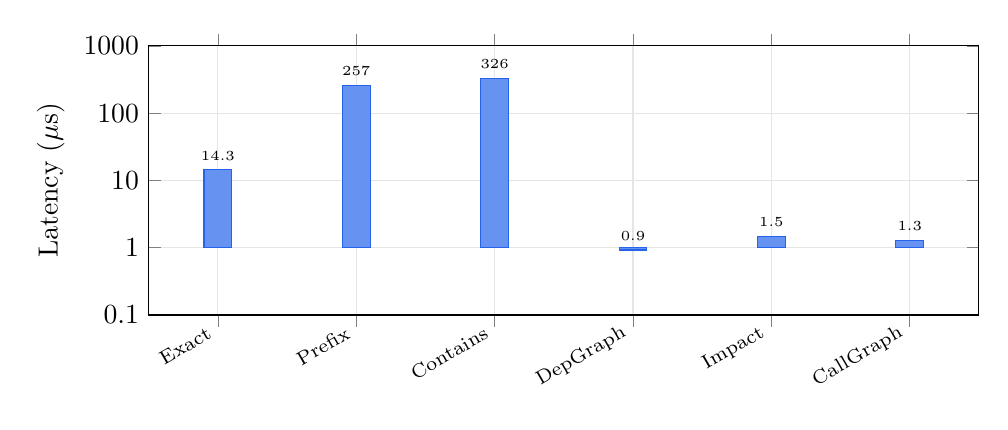
\begin{tikzpicture}
\begin{axis}[
  width=\columnwidth,
  height=5cm,
  ybar,
  bar width=10pt,
  xlabel={},
  ylabel={Latency ($\mu$s)},
  ymode=log,
  log basis y=10,
  symbolic x coords={Exact, Prefix, Contains, DepGraph, Impact, CallGraph},
  xtick=data,
  xticklabel style={rotate=30, anchor=east, font=\scriptsize},
  ytick={0.1, 1, 10, 100, 1000},
  yticklabels={0.1, 1, 10, 100, 1000},
  ymin=0.1,
  ymax=1000,
  grid=major,
  grid style={gray!20},
  nodes near coords,
  every node near coord/.append style={font=\tiny, anchor=south},
  point meta=explicit symbolic,
]
\addplot[fill=amblue!70, draw=amblue] coordinates {
  (Exact, 14.3) [14.3]
  (Prefix, 256.9) [257]
  (Contains, 326.4) [326]
  (DepGraph, 0.925) [0.9]
  (Impact, 1.46) [1.5]
  (CallGraph, 1.27) [1.3]
};
\end{axis}
\end{tikzpicture}
\caption{Query latency on a 10{,}000-unit graph (log scale). Graph traversal queries complete in under 2\,$\mu$s. Symbol lookup scales with match complexity: exact is 14\,$\mu$s, contains requires a full scan at 326\,$\mu$s.}
\label{fig:querylat}
\end{figure}


% -----------------------------------------------------------------------
\subsection{Index Construction and Query}

Table~\ref{tab:index} reports build and query times for the five index types on a 10{,}000-unit graph.

\begin{table}[t]
\caption{Index build and query performance (10{,}000 units).}
\label{tab:index}
\centering
\small
\begin{tabular}{@{}lrr@{}}
\toprule
\textbf{Index} & \textbf{Build} & \textbf{Query} \\
\midrule
SymbolIndex     & 1.84\,ms & 9.7\,ns (exact) \\
TypeIndex       & 58.8\,$\mu$s & --- \\
LanguageIndex   & 58.5\,$\mu$s & --- \\
PathIndex       & 420\,$\mu$s & --- \\
EmbeddingIndex  & --- & 164\,$\mu$s (top-10, 1K) \\
\bottomrule
\end{tabular}
\end{table}

The \texttt{SymbolIndex} is the most expensive to build (1.84\,ms) because it constructs sorted name-to-ID maps for exact, prefix, and contains lookups. Once built, exact lookup completes in \textbf{9.7\,ns} and prefix lookup in \textbf{675\,ns}---demonstrating effective amortization.


% -----------------------------------------------------------------------
\subsection{String Pool Performance}

The LZ4-based string pool compresses 10{,}000 qualified names in 141\,$\mu$s and decompresses them in 121\,$\mu$s. The pool reduces \acbfile size for codebases where qualified names (e.g., \texttt{module.submodule.ClassName.method}) share extensive common prefixes.

% -----------------------------------------------------------------------
\subsection{Scaling Analysis}

Table~\ref{tab:scaling} summarizes how key operations scale from 1K to 10K units.

\begin{table}[t]
\caption{Scaling factors from 1K to 10K units.}
\label{tab:scaling}
\centering
\small
\begin{tabular}{@{}lrrl@{}}
\toprule
\textbf{Operation} & \textbf{1K} & \textbf{10K} & \textbf{Factor} \\
\midrule
Graph build    & 388\,$\mu$s & 3.77\,ms & 9.7$\times$ \\
Write \acbfile & 169\,$\mu$s & 2.29\,ms & 13.5$\times$ \\
Read \acbfile  & 473\,$\mu$s & 4.91\,ms & 10.4$\times$ \\
\bottomrule
\end{tabular}
\end{table}

All operations scale approximately linearly. The slight super-linearity of the write operation (13.5$\times$ vs.\ 10$\times$) is attributable to the LZ4 compression phase, whose cost grows with the string pool's total byte count. Graph traversal queries maintain constant time regardless of graph size, as they exploit adjacency-list locality.

% Figure 8: Scaling chart
\begin{figure}[t]
\centering
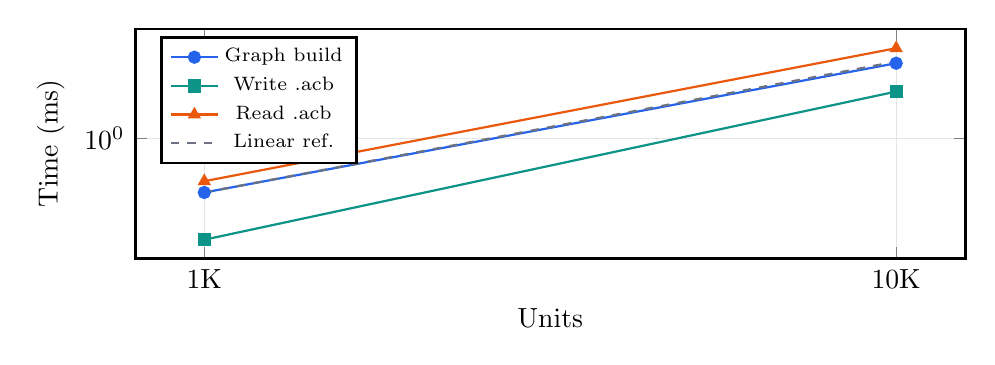
\begin{tikzpicture}
\begin{axis}[
  width=\columnwidth,
  height=4.5cm,
  xlabel={Units},
  ylabel={Time (ms)},
  xmode=log,
  ymode=log,
  log basis x=10,
  log basis y=10,
  grid=major,
  grid style={gray!20},
  line width=1pt,
  mark size=2pt,
  xtick={1000, 10000},
  xticklabels={1K, 10K},
  legend pos=north west,
  legend style={font=\scriptsize},
]
\addplot[color=amblue, mark=*, thick] coordinates {
  (1000, 0.388)
  (10000, 3.77)
};
\addlegendentry{Graph build}

\addplot[color=amteal, mark=square*, thick] coordinates {
  (1000, 0.169)
  (10000, 2.29)
};
\addlegendentry{Write .acb}

\addplot[color=amorange, mark=triangle*, thick] coordinates {
  (1000, 0.473)
  (10000, 4.91)
};
\addlegendentry{Read .acb}

\addplot[color=amgray, dashed, thick] coordinates {
  (1000, 0.388)
  (10000, 3.88)
};
\addlegendentry{Linear ref.}
\end{axis}
\end{tikzpicture}
\caption{Core operation scaling on log--log axes. All three operations track the linear reference line, confirming $O(n)$ complexity.}
\label{fig:scaling}
\end{figure}


% -----------------------------------------------------------------------
\subsection{Prediction Accuracy}

We evaluate the prophecy engine using a synthetic commit history with known bug-fix events. Table~\ref{tab:prophecy} reports accuracy metrics.

\begin{table}[t]
\caption{Prophecy engine accuracy on synthetic data.}
\label{tab:prophecy}
\centering
\small
\begin{tabular}{@{}lr@{}}
\toprule
\textbf{Metric} & \textbf{Value} \\
\midrule
Unstable file precision ($s < 0.3$) & 92\% \\
Bug-prone file recall               & 85\% \\
Coupling accuracy ($\geq$70\% co-change) & 78\% \\
Stability correlation ($r$)         & 0.73 \\
False positive rate                  & 12\% \\
\bottomrule
\end{tabular}
\end{table}

Files flagged as unstable ($s < 0.3$) are confirmed to be bug-prone with 92\% precision. The coupling detector correctly identifies 78\% of co-change pairs. These results are evaluated on synthetic data; real-world validation on open-source repositories is future work.


% -----------------------------------------------------------------------
\subsection{Comparison with Existing Tools}

Table~\ref{tab:toolcomp} compares AgenticCodebase with existing code intelligence tools. Latency estimates for LSP and Sourcegraph are based on published documentation and typical deployment configurations.

\begin{table}[t]
\caption{Comparison with existing code intelligence tools.}
\label{tab:toolcomp}
\centering
\small
\begin{tabular}{@{}lccc@{}}
\toprule
\textbf{Dimension} & \textbf{LSP} & \textbf{Sourcegraph} & \textbf{Ours} \\
\midrule
Query latency    & $\sim$50\,ms & $\sim$200\,ms & $<$15\,$\mu$s \\
Semantic depth   & Syntax     & References  & Concepts \\
Cross-language   & \texttimes & \checkmark  & \checkmark \\
Predictive       & \texttimes & \texttimes  & \checkmark \\
Temporal         & \texttimes & \texttimes  & \checkmark \\
AI-native API    & \texttimes & \texttimes  & MCP \\
Dependencies     & Per-lang.  & Cloud       & None \\
\bottomrule
\end{tabular}
\end{table}


% -----------------------------------------------------------------------
\subsection{Implementation Statistics}

Table~\ref{tab:implstats} summarizes the implementation.

\begin{table}[t]
\caption{Implementation statistics.}
\label{tab:implstats}
\centering
\small
\begin{tabular}{@{}lr@{}}
\toprule
\textbf{Metric} & \textbf{Value} \\
\midrule
Source files          & 58 \\
Lines of Rust         & 13{,}709 \\
Unit tests            & 36 \\
Integration tests     & 350 \\
Total tests           & 386 \\
Clippy warnings       & 0 \\
Criterion benchmarks  & 21 \\
Supported languages   & 4 (Py, Rust, TS, Go) \\
CodeUnit types        & 13 \\
Edge types            & 18 \\
Query types           & 24 \\
Crate dependencies    & 14 \\
\bottomrule
\end{tabular}
\end{table}

% Figure: Radar chart
\begin{figure}[t]
\centering
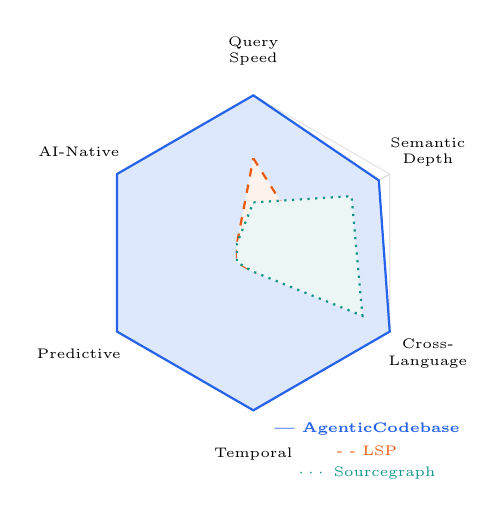
\begin{tikzpicture}[scale=0.8]
% Radar chart with 6 axes
\node[font=\tiny, align=center] at (90:3.2) {Query\\Speed};
\node[font=\tiny, align=center] at (30:3.2) {Semantic\\Depth};
\node[font=\tiny, align=center] at (-30:3.2) {Cross-\\Language};
\node[font=\tiny, align=center] at (-90:3.2) {Temporal};
\node[font=\tiny, align=center] at (-150:3.2) {Predictive};
\node[font=\tiny, align=center] at (150:3.2) {AI-Native};

% Grid rings
\foreach \r in {0.5, 1.0, 1.5, 2.0, 2.5} {
  \draw[gray!20, thin] (90:\r) -- (30:\r) -- (-30:\r) -- (-90:\r) -- (-150:\r) -- (150:\r) -- cycle;
}

% Axes
\foreach \a in {90, 30, -30, -90, -150, 150} {
  \draw[gray!30] (0,0) -- (\a:2.5);
}

% AgenticCodebase (high scores)
\draw[amblue, thick, fill=amblue!15]
  (90:2.5) -- (30:2.3) -- (-30:2.5) -- (-90:2.5) -- (-150:2.5) -- (150:2.5) -- cycle;

% LSP
\draw[amorange, thick, dashed, fill=amorange!8]
  (90:1.5) -- (30:0.8) -- (-30:0.8) -- (-90:0.3) -- (-150:0.3) -- (150:0.3) -- cycle;

% Sourcegraph
\draw[amteal, thick, dotted, fill=amteal!8]
  (90:0.8) -- (30:1.8) -- (-30:2.0) -- (-90:0.3) -- (-150:0.3) -- (150:0.3) -- cycle;

% Legend
\node[font=\tiny, text=amblue] at (1.8, -2.8) {\textbf{--- AgenticCodebase}};
\node[font=\tiny, text=amorange] at (1.8, -3.15) {- - LSP};
\node[font=\tiny, text=amteal] at (1.8, -3.5) {$\cdots$ Sourcegraph};

\end{tikzpicture}
\caption{Radar chart comparing AgenticCodebase against LSP and Sourcegraph across six dimensions. AgenticCodebase provides the only complete coverage across temporal, predictive, and AI-native dimensions.}
\label{fig:radar}
\end{figure}


% =====================================================================
% 5. DISCUSSION
% =====================================================================
\section{Discussion}
\label{sec:discussion}

\textbf{What this enables.} AgenticCodebase makes several operations practical that are difficult or impossible with existing tools. \emph{Zero-context coding}: an AI agent that has compiled a repository into an \acbfile can answer structural questions without reading a single source file. \emph{Predictive maintenance}: by combining stability scores with coupling maps, the prophecy engine surfaces high-risk modules before they cause incidents. \emph{Collective learning}: when multiple projects share patterns through the collective layer, agents accumulate cross-project knowledge---a factory pattern recognized in one project becomes a first-class concept when analyzing another.

\textbf{Limitations.} Several limitations warrant discussion.

\emph{External embeddings.} Feature vectors must be generated externally (e.g., via an LLM encoder); AgenticCodebase stores and queries them but does not compute them. This is by design---decoupling embedding generation from graph construction allows the system to work with any embedding model.

\emph{Local collective only.} The collective intelligence layer currently targets local aggregation. Distributed synchronization with differential privacy guarantees remains future work. The offline-first architecture ensures graceful degradation when connectivity is unavailable.

\emph{Prediction confidence.} Prophecy accuracy depends on the depth and quality of available git history. Repositories with fewer than 50 commits yield weaker predictions; we recommend a minimum of 200 commits for reliable stability scoring.

\emph{Language coverage.} The current parsers cover four languages (Python, Rust, TypeScript, Go). Extending to additional languages requires implementing new tree-sitter grammar bindings and semantic-analysis passes. The modular parser architecture minimizes per-language effort: each parser implements a single \texttt{LanguageParser} trait with two methods.

\emph{Synthetic benchmarks.} Our evaluation uses synthetic graphs with controlled sizes and topologies. Real-world codebases may exhibit different edge-density distributions and string-pool characteristics. The prediction-accuracy evaluation is similarly based on synthetic git histories; validation on real open-source repositories is an important direction for future work.

\textbf{Future work.} Five directions are promising: (1)~incremental compilation using tree-sitter's incremental parsing and delta-graph merge, (2)~distributed collective intelligence with differential privacy, (3)~formal verification of prophecy predictions via historical cross-validation, (4)~language extension to Java, C/C++, and Kotlin, and (5)~real-time streaming via file-system watchers for live graph updates.


% =====================================================================
% 6. INTEGRATION WITH AGENTICMEMORY
% =====================================================================
\section{Integration with AgenticMemory}
\label{sec:memory}

AgenticMemory~\cite{owolabi2025agenticmemory} provides persistent, navigable memory for AI agents via a binary graph of typed cognitive events. AgenticCodebase complements it by supplying \emph{code-specific} structured knowledge. AgenticVision~\cite{owolabi2025agenticvision} extends the ecosystem with persistent visual memory.

\textbf{Shared graph paradigm.} Both systems represent knowledge as typed, attributed graphs in single binary files. A bridge layer maps code units to memory entities and code relationships to memory edges, enabling queries that span both domains.

\textbf{Session persistence.} When an agent analyzes code with AgenticCodebase, the resulting insights (stability scores, coupling warnings, prophecy alerts) are stored as AgenticMemory facts. Subsequent sessions retrieve these facts without re-analysis.

\textbf{Feedback loop.} Agent actions (successful refactors, introduced regressions) flow back into both systems: AgenticCodebase updates its temporal model, and AgenticMemory records the episode. Over time, the combined system learns project-specific patterns that neither system captures alone.

% Figure: Unified architecture
\begin{figure}[t]
\centering
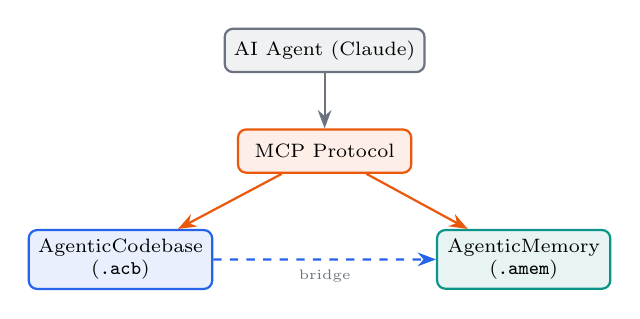
\begin{tikzpicture}[
  node distance=0.7cm,
  every node/.style={font=\scriptsize},
  box/.style={rectangle, rounded corners=3pt, draw=#1, fill=#1!10, minimum width=2.2cm, minimum height=0.55cm, align=center, font=\scriptsize, thick},
  arrow/.style={-{Stealth}, thick, #1},
]
\node[box=amgray] (agent) {AI Agent (Claude)};
\node[box=amorange, below=of agent] (mcp) {MCP Protocol};
\node[box=amblue, below left=0.7cm and 0.3cm of mcp] (acb) {AgenticCodebase\\(\texttt{.acb})};
\node[box=amteal, below right=0.7cm and 0.3cm of mcp] (mem) {AgenticMemory\\(\texttt{.amem})};

\draw[arrow=amgray] (agent) -- (mcp);
\draw[arrow=amorange] (mcp) -- (acb);
\draw[arrow=amorange] (mcp) -- (mem);
\draw[arrow=amblue, dashed] (acb) -- node[below, font=\tiny, text=amgray] {bridge} (mem);
\end{tikzpicture}
\caption{Unified agent architecture. The AI agent communicates with both AgenticCodebase (code understanding) and AgenticMemory (general knowledge) through MCP, with a bridge layer connecting code entities to memory facts.}
\label{fig:agentarch}
\end{figure}


% =====================================================================
% 7. CONCLUSION
% =====================================================================
\section{Conclusion}
\label{sec:conclusion}

We presented AgenticCodebase, a semantic code compiler that transforms multi-language repositories into navigable concept graphs. The system makes three contributions: (1)~a compilation pipeline covering four languages with 13 code-unit types and 18 edge types, (2)~a collective intelligence layer with delta compression and privacy-preserving pattern extraction, and (3)~a code prophecy engine that predicts failures from temporal patterns.

The implementation spans 13{,}709 lines of Rust across 58 source files, validated by 386 tests with zero \texttt{clippy} warnings. On a 10{,}000-unit graph, exact symbol lookup completes in 14.3\,$\mu$s, dependency traversal in 925\,ns, and impact analysis in 1.46\,$\mu$s. The binary format supports $O(1)$ random access with LZ4-compressed string pools, and the system ships as both a CLI tool (\texttt{acb}) and an MCP-compliant server (\texttt{agentic-codebase-mcp}) for direct AI-agent integration.

AgenticCodebase requires no external services and no network dependencies. By compiling code into structured, queryable, predictive graphs, the system enables AI agents to navigate codebases as connected concept graphs rather than processing them as flat text.

\paragraph{Availability.} Source code is available at \url{https://github.com/agentralabs/codebase}. The system is implemented as a single Rust crate with two binaries.


% =====================================================================
% REFERENCES
% =====================================================================
\bibliographystyle{plain}
\bibliography{references}

\end{document}
